\subsection{Expanding our method with glia cells}
Modeling the equation in one dimension is done by considering the points $a$ and $b$, and the line between them.  In this case, $a$ is the axon side and $b$ is the dendrite side.  Due to this, the boundary conditions for $a$ and $b$ differ.  For $a$, we have 
\begin{align*}
\kappa \nabla c &= -{k}_3cP^T + {k}_4(1-P^T),
\end{align*}
and for $b$ we have
\begin{align*}
\kappa \nabla c &= -{k}_1c P^R + {k}_2(1-P^R).
\end{align*}
The next step is to combine these boundary conditions with the modeling equation to form a set of ODE's.

%\subsection*{Mass matrix}
%The mass matrix was found to be \\
%\\
%$
%M_{N,N} =
% \begin{bmatrix}
%  \frac{h}{3}       & \frac{h}{6}    & 0           & \cdots           & \cdots           & 0 \\
%  \frac{h}{6}       & \frac{2h}{3}   & \ddots      & \ddots           & \cdots           & \vdots \\
%  0                 & \ddots         & \ddots      & \ddots           & \ddots           & \vdots  \\
%  \vdots            & \ddots         & \ddots      & \ddots           & \ddots           & 0  \\
%  \vdots            & \vdots         & \ddots      & \ddots           & \frac{2h}{3}     & \frac{h}{6}  \\
%  0                 & \cdots         & \cdots      & 0                & \frac{h}{6}      & \frac{h}{3}
% \end{bmatrix},\\
%$
%while the stiffness matrix was\\
%$
%K_{N,N} =
% \begin{bmatrix}
%  \frac{1}{h}        & -\frac{1}{h}    & 0           & \cdots           & \cdots            & 0 \\
%  -\frac{1}{h}       & \frac{2}{h}     & \ddots      & \ddots           & \cdots            & \vdots \\
%  0                  & \ddots          & \ddots      & \ddots           & \ddots            & \vdots  \\
%  \vdots             & \ddots          & \ddots      & \ddots           & \ddots            & 0  \\
%  \vdots             & \vdots          & \ddots      & \ddots           & \frac{2}{h}       & -\frac{1}{h}  \\
%  0                  & \cdots          & \cdots      & 0                & -\frac{1}{h}      & \frac{1}{h}
% \end{bmatrix}.\\
%$

Using the finite element method the final system of equations then becomes

\begin{align*}
M \dot{C}(t) =  &-KC(t) - k_3Q^a(P_a^T(t))C_1(t) + \left[k_4(1-P_a^T(t))\right]d^a \\
& - k_1Q^b(P_b^R(t))C_N(t) + \left[k_2(1-P_b^R(t))\right]d^b \\
\frac{\partial P_a^T(t)}{dt} &= -ck_3 P_a^T(t) + (k_4 + k_5)(1-P_a^T(t))\\
\frac{\partial P_b^R(t)}{dt} &= -ck_1 P_b^R(t) + k_2(1-P_b^R(t)),
\end{align*}
where $P_a^T(t)$ defines the probability that a transporter in side $a$ is available and $P_b^R(t)$ defines the probability that a receptor in side b is available at time $t$. $M$ is the problem mass matrix and $K$ is the problem stiffness matrix. $C$ is the concentration of neurotransmitters at all internal nodes.

The system was found by Jörg Henrik Holstad \cite{holstad} and was solved by combining into one large system and solved by using Matlab's ode45.

A plot using N = 6 internal nodes is shown in figure \ref{fig:1dode}. More realistic constant values could be trued here as well. 

\begin{figure}[ht]
  \centering
    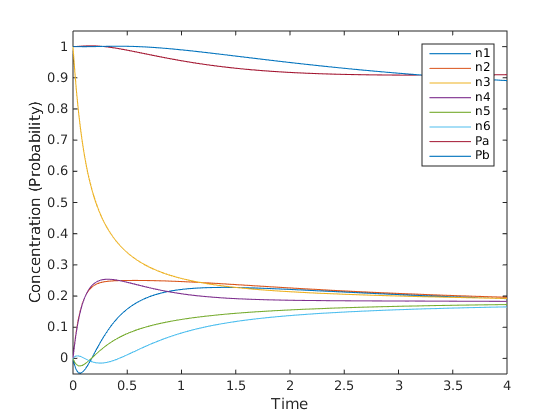
\includegraphics[width=0.45\textwidth]{1dodeLabels}
      \caption{Solving the one dimensional case using the element method and Matlab's ode45 using the constants $a = 0$, $b = 8$, $N = 6$, $\kappa = 3$, $k_1=k_2=k_3=k_4=k_5 = 0.5$, $P_a^T(0) = P_b^R(0) = 1$, $C(0) = [0, 0, 1, 0, 0, 0]$.}
      \label{fig:1dode}
\end{figure}

The 2D scheme from \cite{holstad} was also tried, but as shown in figure \ref{fig:2dode45} we couldn't get the scheme to be stable.

\begin{figure}[ht]
    \centering
    \begin{subfigure}[b]{0.45\textwidth}
        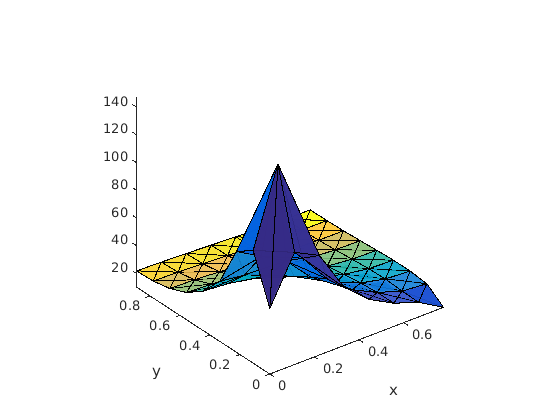
\includegraphics[width=\textwidth]{2dode45}
        \caption{2D solution at time 0.3 in a rectangular domain.}
    \end{subfigure}
    ~ 
    \begin{subfigure}[b]{0.45\textwidth}
        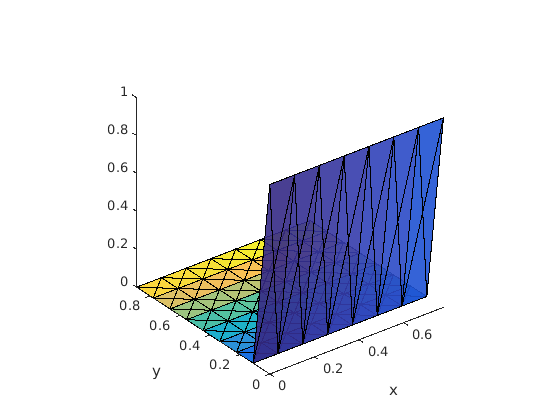
\includegraphics[width=\textwidth]{2dode45initial}
        \caption{Initial condition in a rectangular domain.}
    \end{subfigure} 
    \caption{Our try to solve the 2D model with the finite element method and Matlab's ode45. We recognize that the scheme is numerically unstable and blows up. }
    \label{fig:2dode45}
\end{figure}

